\documentclass[11pt]{article}

\usepackage{common}
\usepackage{booktabs}
\title{The Analytics Edge, Final Report:\\ Building an Article Recommender for Bleacher Report Basketball}
\author{for Professor Dimitris Bertsimas and Emma Gibson \text{ } \\ \\ by Stephen Albro \& Cyrille Combettes \\ salbro@mit.edu, cyrille@mit.edu}
\begin{document}
\maketitle{}


\section{Abstract}

\section{Motivation and Project Abstract}
As avid basketball fans, we have enjoyed reading a variety of NBA articles to keep up-to-date on the league during our busy year in the MBAn program.  Bleacher Report, a primary digital destination for sports article readers, contains well written articles covering the league, and competes as advertisement real-estate with the likes of ESPN.com, FoxSports.com, CBSSports.com, SBNation.com, and others. \\

  In an age of cut-throat digital competition, it is vital for websites to be able to retain visitors. The hope for a Bleacher Report article reader is two-fold. First, that the visitor jumps from article to article \textit{on the website}, rather than returning to the search engine results page.  Second, that the visitor falls in love with the content and coverage of Bleacher Report's articles, and develops a loyalty to the website. \\

We feel that having a micro targetted article recommendation system would provide Bleacher Report with an analytics-based edge over its competitors, since well targeted articles could increase the chances of prolonged visits, and increase website loyalty by making users feel known.  In this paper, we develop a prototype for an article recommendation system using state of the art natural language processing techniques for both cleaning and analyzing bleacher report articles.  Specifically, we aim to cluster over 3000 Bleacher Report articles by testing three different approaches: Topic Modeling, Word2Vec text embeddings, and NMF (CYRILLE WRITE OUT FULL NAME AND TALK ABUOT WHAT NMF IS).  \{GO INTO MORE DETAIL HERE ABOUT HOW CLUSTER HELPS THE RECOMMENDER. \}

% To improve user affinity for Bleacher Report, we even include AI-generated articles, which employ recurrent neural networks trained on our corpus. 

\section{Data Collection and Cleaning}
\subsection{Data Collection}
Bleacher Report does not provide easy access to their articles in a public database.  However, News API is a company that provides API access to major news articles from a variety of sources, and this access is free for non-commercial projects. Using NewsAPI, we queried Bleacher Report NBA articles from October 17, the start of the 2017-2018 NBA season. Our entire query consisted of joining words like basketball and NBA with all 30 teams and the top 25 active players.  In the end, we received 3314 URLs (with their corresponding authors, titles, and other metadata) in return.  We then wrote a script to request the webpage for each URL and scrape its content, picking the paragraphs out of the HTML.

\subsection{Data Cleaning}
In the real world, data is never clean, and this is magnified in the case of textual data. There were a number of preprocessing steps we had to do before our articles were ready for analysis. In our cleaning efforts, we made decisions \textit{based on the purpose of our task} - to cluster documents for better recommendation power.  In particular, a bag-of-words approach to cleaning was preferred over one that preserved punctuation and grammar.  \\

\subsubsection{Punctuation Removal, Initial Stopwords, and Lowercasing}
First, we tokenized each article. In natural language processing, tokenizing is a way of chopping up a document into pieces, the most obvious way being to tokenize by \textit{word}, which is what we initially did.  Next we discarded any non-alphabetical tokens (e.g. 8pm, 704, !, .), and converted every token to lower case.  After converting everything to lower case, we did our first round of stop word removal (we remove more later).  In  NLP a stop word is any word that you remove because its insignificant for your application. In this first round, we removed basic articles (the, a) and about 170 other words deemed insignificant by Python's Natural Language Toolkit, mostly personal pronouns and simple verbs.

\subsubsection{Specialized NBA Tokenization}
Next, since we were analyzing NBA articles, we had to take into account the fact that each player (and each team for that matter) can be referred to in a variety of ways. For example, the NBA superstar LeBron James can be called LeBron James, LeBron, Bron, or James, and the Boston Celtics might be formally referred to as such in the title, but in the article's body they might just be Boston. For this reason, we compiled lists of team names, players, and coaches.  For each article, we replaced all forms of each entity with its underscored full version, so that for example LeBron James would always be lebron\_james, no matter if he occurred as Bron, James, or Lebron in a given sentence.  At times it was necessary to infer from ambiguous usage. We concluded that, for example, the word \textit{Boston} should be replaced by boston\_celtics only if the entire phrase Boston Celtics appeared somewhere in the article.  This specialized, application-specific tokenization step allowed us to capture much more information about each superstar/team/coach than would for example, treating Bron as a separate player as Lebron. \\

\subsubsection{Stemming Each Word}
Next, we needed to address the fact that sometimes the same words take different forms. A reasonable assumption that we made the words playing, played, play, and plays all capture the same information as far as topic modeling goes. Thus we decided to \textit{stem} each word, which in NLP means to convert every word into its root form.  Python's Natural Language Toolkit provides a stemmer.

[ IF I LIKE THESE RESULTS BETTER REDO THE TRIMMING SECTION TO UPDATE TO NEW NUMBERS OF WORDS]

\subsubsection{Trimming Down the Vocabulary}
A model is only as good as its input, and so as a last step, we realized that we needed to trim down the vocabulary of our articles. In NLP, a \textit{vocabulary} is simply the complete set of words that the model knows about.  We already removed basic stop words, but figured that many more could be removed. For clustering documents, its important to identify information-containing words (player and team names, high-impact verbs, league terminology), and less important to identify mundane nouns and verbs (table, cup, gave, took) even if their not considered stop words. \\

To identify our functional vocabulary, we used a \textit{document frequency} approach. The document frequency of a given word is simply the fraction of documents (in this case articles) that the word appears in. The word \textit{the}, for example, has a document frequency of 1.0. If a word occurs too \textit{infrequently}, it is probably a unique name or an article-specific entity, and thus unhelpful in forming clusters. On the other hand, if a word occurs too \textit{frequently}, it is probably a common word and thus contains very little information related to topics.  \\

Thus, we sought lower and upper document frequency cutoffs for including a word in the vocabulary.  As a sanity check, we knew our upper cutoff had to be at least high than the document frequency of LeBron James (0.22, he the most famous superstar), since every player should be in our vocabulary. After seeing irrelevant words present with an upper cutoff of even 0.5, we knew that the upper cutoff had to be lower than that, and decided upon 0.35 after experimentation (at this point the eye test was possible). Our lower cutoff was 0.01, which means that if a word appeared in less than 34 out of 3314 total articles, it was discarded.  In total, the new vocabulary consisted of about 3500 tokens with document frequencies within the range (0.01, 0.35), including the major players and teams, and, we think, the important, topic-filled sports and NBA terminology. To give a sense, some of the first few tokens printed from our vocab set include \textit{son, statistics, honor, turnover, athleticism, pulled, dribble, andrew\_wiggins, offseasons, attitude, cuts,} and \textit{jump}.  


\section{Methods}
In order to produce a quality article recommendation, it is necessary to be able to identify similar documents (articles).  If we can find a way to do this, we have a strategy for producing recommendations to a new website visitor: After observing which articles she reads, simply recommend the most \textit{similar} articles that she has not read yet.\\

In the following section, define \\
$D = \{d_1, d_2, ... d_N \}, \quad$ the set of $N$ documents (articles) obtained from Bleacher Report \\
$V = \{w_1, w_2, ... w_M \}, \quad$ the set of $M$ words in the final vocabulary \\
$T = \{t_1, t_2, ..., t_K\}, \quad$ the set of $K$ topics in the documents \\

\subsection{Topic Modeling with Latent Dirichlet Allocation}
\subsubsection{Background}
The first way we approached the question of document similarity was topic modeling.  In topic modeling, we attempt to infer which \textit{topics} are present among the documents, and then after that, to identify which topics belong to each particular document, and in what proportion.  Here a \textit{topic} is simply a probability distribution over the words in the vocabulary.  For each topic, each word has a probability of being chosen.  The task is difficult, because we are trying \textit{both} to infer the topics themselves (all we provide in advance is $K$, the number of topics), \textit{as well as} the topic-composition of each document. \\

We decided upon a specific Topic Model known as Latent Dirichlet Allocation (LDA). LDA assumes that documents are created according to the following generate process: \\
$\text{} \quad$ 1. Randomly generate a distribution over topics\footnote{requires a distribution over a distribution, will leave this for the appendix}. \\
$\text{} \quad$ 2. To come up with each word in the document: \\
$\text{} \quad$ $\quad$ a. Randomly choose a topic. \\
$\text{} \quad$ $\quad$ b. Randomly choose a word from that topic.  \\

The main task of LDA is then to infer two parameters: \\
$\beta_t$: the distribution over words for topic $t$: $\mathcal{P}(w | t) \quad \forall w \in V$ \\
$\theta_{dt}$: the proportion of document $d$ that came from topic $t$: $\mathcal{P}(t | d) \quad \forall t \in T$ \\

LDA infers these parameters according to which values make the data the most likely. \\

These estimates allow us to express each document as a vector, which is a distribution over the topics it contains.  The vectorized documents can then be clustered based on their topical composition. The idea is that if I love the topic of statistics and I also love the topic of Lebron James, I will be recommended articles about Lebron James' statistics. 

This is a bag-of-words model because the generative story says nothing about grammar. For topic modeling, we do not care about grammar anyway.    

\subsubsection{Approach}
We trained LDA models on the cleaned Bleacher Report articles using Python's sklearn libraries.  When training the models, two hyper-parameters needed to be fine-tuned. The first was $K$, the number of topics to ask for.  The second was $\gamma$, the learning rate of the solver.  (TALK MORE ABOUT THIS?). We decided to use a grid search cross validation approach. Since topic modeling is an unsupervised problem, there was no need for a separate validation set.  Instead we used the log-likelihood of the trained model as our measure of model quality. 

We found that for $k \in \{10, 15, 20, 25, 30\}$ and $\gamma \in \{.5, .7, .9\}$ the best hyper-parameters were $k=10$, $\gamma = 0.7$. (SEARCH LOWER VALUES OF K??)\\

(DO THIS ON OTHER VALUES SO ITS NOT EXACTLY THE SAME AS BLOG TUTORIAL ??)


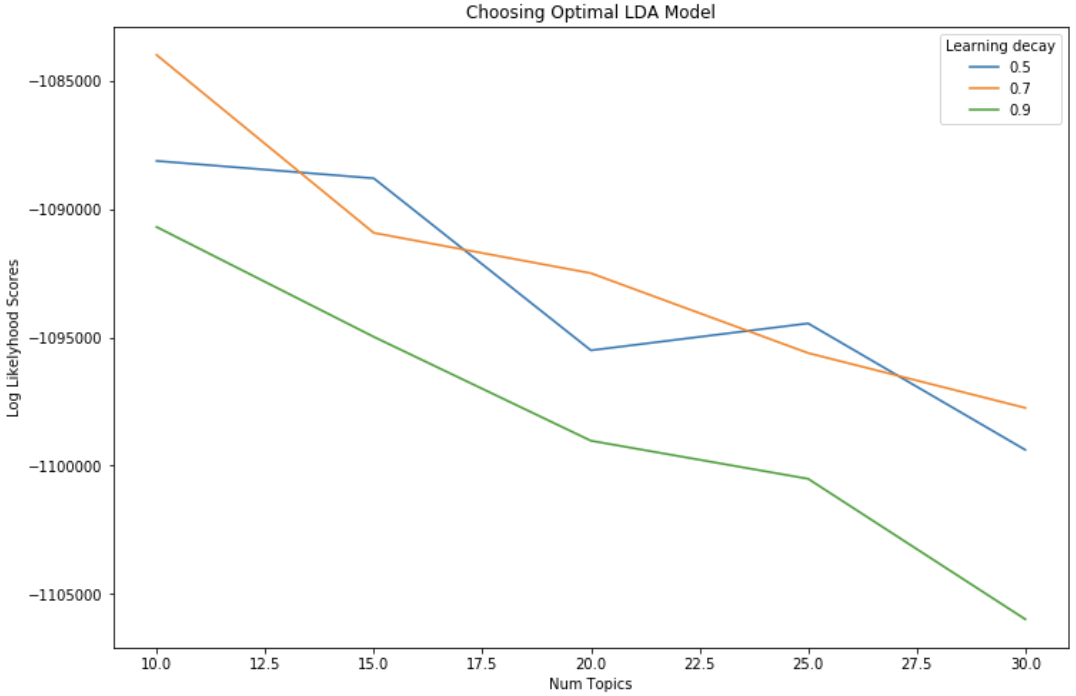
\includegraphics{gridsearch.png} \\
We were very pleased with the results of our model, which we visualized using Python's LDAvis library tools. 
The visualization has two components. First, it projects each cluster onto the first two principal components of the document vector space, and shows the position of the clusters in the resulting 2D graph.   (FIX THIS DESCRIPTION IT MIGHT NOT BE ACCURATE... FIGURE OUT EXACTLY WHAT THAT PICTURE IS SHOWING). When you hover over a topic, the top 30 words for that topic are shown in decreasing order. 

RESULT 1 PIC \\ 
RESULT 2 PIC\\ 
RESULT 3 PIC\\

...\\

RESULT N PIC \\




(SHOW SIMILAR HEADLINES OF EACH TOPIC)


(TRY IT ON A NEW ARTICLE FROM THE PAST DAY, which we don't have in our data set)


Our first approach to document clustering 
- summary: topic model (definition) to cluster
- clusters (show and interpret)
- place each document that someone sees as a combination of clusters ... find KNN and use the code thing


\subsection{<METHOD 2>}
% To obtain similarity between documents, we decided to cluster the documents or if we can successfully embed each document in a vector space, we can reason about which documents are similar. 

\subsection{<METHOD N>}



\section{Discussion}
\subsection{Which Approach is Best}
- how to we measure success, etc.

\subsection{Why This Project Was Important}
- we learned a lot about all three methods
- most of the world's data is text \\
- lots of online advertising \\
- lot of research in NLP because anlytics provides an edge \\




\end{document}